\documentclass[11pt]{article}

\usepackage{latexsym}
\usepackage{graphicx}
\usepackage{amssymb}
\usepackage{amsthm}
\usepackage{enumerate}
\usepackage{amsmath}
\usepackage{cancel}
\numberwithin{equation}{section}

\setlength{\evensidemargin}{.25in}
\setlength{\oddsidemargin}{-.25in}
\setlength{\topmargin}{-.75in}
\setlength{\textwidth}{6.5in}
\setlength{\textheight}{9.5in}
\newcommand{\due}{March 3rd, 2016}
\newcommand{\HWnum}{6}
\newcommand{\grad}{\bold\nabla}
\newcommand{\vecE}{\vec{E}}
\newcommand{\scrptR}{\vec{\mathfrak{R}}}
\newcommand{\kapa}{\frac{1}{4\pi\epsilon_0}}
\newcommand{\emf}{\mathcal{E}}
\newcommand{\unit}[1]{\ensuremath{\, \mathrm{#1}}}
\newcommand{\real}{\textnormal{Re}}
\newcommand{\Erf}{\textnormal{Erf}}
\newcommand{\sech}{\textnormal{sech}}
\newcommand{\scrO}{\mathcal{O}}
\newcommand{\levi}{\widetilde{\epsilon}}
\newcommand{\partiald}[2]{\ensuremath{\frac{\partial{#1}}{\partial{#2}}}}
\newcommand{\norm}[2]{\langle{#1}|{#2}\rangle}
\newcommand{\inprod}[2]{\langle{#1}|{#2}\rangle}
\newcommand{\ket}[1]{|{#1}\rangle}
\newcommand{\bra}[1]{\langle{#1}|}





\begin{document}
\begin{titlepage}
\setlength{\topmargin}{1.5in}
\begin{center}
\Huge{Physics 3320} \\
\LARGE{Principles of Electricity and Magnetism II} \\
\Large{Professor Ana Maria Rey} \\[1cm]

\huge{Homework \#\HWnum}\\[0.5cm]

\large{Joe Becker} \\
\large{SID: 810-07-1484} \\
\large{\due} 

\end{center}

\end{titlepage}




\section{Problem \#1}
\begin{enumerate}[(1)]
\item To calculate the change in energy of an electron gas at zero temperature due to a 
magnetic field, $H$, we note that the Fermi-Dirac distribution becomes
$$f(\varepsilon) = \frac{1}{e^{(\varepsilon\pm\mu_BH-\mu)/T}+1}$$
where $\mu_B$ is the Bohr magneton which is given by
$$\mu_B = \frac{e\hbar}{2mc}$$
Note that the positive $\mu_BH$ is related to the state where the spin is parallel to the
magnetic field and the negative $\mu_BH$ is the anti-parallel case.  Using $f(\varepsilon)$ 
and the density of states, $\nu(\varepsilon)$, for a spin $\frac{1}{2}$ particle given as
$$\nu(\varepsilon) = \frac{V}{2\pi^2}\left(\frac{2m}{\hbar^2}\right)^{3/2}\varepsilon^{1/2}$$
we can calculate the energy of the spin up state as temperature goes to zero noting that
$f(\varepsilon)$ becomes the step function. Therefore
\begin{align*}
E_{\uparrow} = \int_{0}^{\infty}\varepsilon\nu(\varepsilon)f(\varepsilon)d\varepsilon &= \frac{V}{4\pi^2}\left(\frac{2m}{\hbar^2}\right)^{3/2}\int_{0}^{\infty}\frac{\varepsilon^{3/2}}{e^{(\varepsilon+\mu_BH-\mu)/T}}d\varepsilon\\
&= \frac{V}{2\pi^2}\left(\frac{2m}{\hbar^2}\right)^{3/2}\int_{0}^{\mu-\mu_BH}\varepsilon^{3/2}d\varepsilon\\
&= \frac{V}{5\pi^2}\left(\frac{2m}{\hbar^2}\right)^{3/2}(\mu-\mu_BH)^{5/2}
\end{align*}
The same follows for the spin down energy just with the change in sign.
$$E_{\downarrow} = \frac{V}{5\pi^2}\left(\frac{2m}{\hbar^2}\right)^{3/2}(\mu+\mu_BH)^{5/2}$$
This implies that the total energy is
$$E = E_{\uparrow} + E_{\downarrow} = \frac{V}{5\pi^2}\left(\frac{2m}{\hbar^2}\right)^{3/2}\left((\mu-\mu_BH)^{5/2} + (\mu+\mu_BH)^{5/2}\right)$$
Therefore we can find the magnetization, $M$, by taking the derivative with respect to $H$
\begin{align*}
M &= \partiald{E}{H} = \frac{V}{2\pi^2}\left(\frac{2m}{\hbar^2}\right)^{3/2}\mu_B\left((\mu+\mu_BH)^{3/2} - (\mu-\mu_BH)^{3/2}\right)
\end{align*}
Note we can take $\mu=\varepsilon_F$ and assume that $\mu_BH<<\varepsilon_F$ which allows us
to expand about $B=0$ to yield
\begin{align*}
M &= \frac{V}{2\pi^2}\left(\frac{2m}{\hbar^2}\right)^{3/2}\mu_B\left((\varepsilon_F+\mu_BH)^{3/2} - (\varepsilon_F-\mu_BH)^{3/2}\right)\\
&= \frac{V}{2\pi^2}\left(\frac{2m}{\hbar^2}\right)^{3/2}\mu_B\left(\mu_B\varepsilon_F^{1/2}H + \mu_B\varepsilon_F^{1/2}H\right)\\
&= 3\frac{V}{2\pi^2}\left(\frac{2m}{\hbar^2}\right)^{3/2}\varepsilon_F^{1/2}\mu_B^2H\\
&= 3\nu(\varepsilon_F)\mu_B^2H
\end{align*}
Note this matches from the direct calculation by using number of states except for the factor
of 3.

\item We can repeat this process for low temperature $T<<\varepsilon_F$ by noting the 
approximation to second order in $T$ is as 
\begin{align*}
E_{\uparrow} &= \frac{V}{5\pi^2}\left(\frac{2m}{\hbar^2}\right)^{3/2}\left((\mu-\mu_BH)^{5/2} + \frac{5{\pi}T^2}{8}(\mu-\mu_BH)^{1/2}\right)\\
E_{\downarrow} &= \frac{V}{5\pi^2}\left(\frac{2m}{\hbar^2}\right)^{3/2}\left((\mu+\mu_BH)^{5/2} + \frac{5{\pi}T^2}{8}(\mu+\mu_BH)^{1/2}\right)
\end{align*}
We can see that the first term yields the $T=0$ solution found in part (a). So to find the
correction for low temperature we take the term of order $T^2$ to find
\begin{align*}
E^{(2)} &= \frac{VT^2}{8\pi}\left(\frac{2m}{\hbar^2}\right)^{3/2}\left((\mu+\mu_BH)^{1/2} + (\mu-\mu_BH)^{1/2}\right)\\
&\Downarrow\\
M^{(2)} = \partiald{E^{(2)}}{H} &= \frac{VT^2\mu_B}{16\pi}\left(\frac{2m}{\hbar^2}\right)^{3/2}\left((\mu+\mu_BH)^{-1/2} - (\mu-\mu_BH)^{-1/2}\right)\\
&\Downarrow\\
&\approx  -\frac{VT^2\mu_B^2H}{16\pi}\left(\frac{2m}{\hbar^2}\right)^{3/2}\epsilon_F^{-3/2}\\
& -\frac{\pi}{8}\left(\frac{T}{\epsilon_F}\right)^{2}\nu(\epsilon_F)\mu_B^2H
\end{align*}
So the corrected magnetization is 
$$M = \nu(\epsilon_F)\mu_BH\left(3 - \frac{\pi T^2}{8\epsilon_F^2}\right)$$
which yields the corrected susceptibility as
$$\chi = \partiald{M}{H} = \nu(\epsilon_F)\mu_B\left(3 - \frac{\pi T^2}{8\epsilon_F^2}\right)$$
Note as we expect an increase in temperature decreases the magnetization and susceptibility. 
\end{enumerate}

\pagebreak

\section{Problem \#2}
\begin{enumerate}[(1)]
\item For a degenerate electronic gas in an external magnetic field there exists orbital 
motion. We assume without loss of generality that the magnetic field points in the $\hat{z}$ 
direction. This implies that there are two types of motion one being in the direction of 
the magnetic field and the other being the circular precession within the perpendicular 
($xy$) plane. Using this fact we can calculate the density of states by noting that in the
presence of a magnetic field the energy energy levels are
$$\varepsilon = \frac{p_z^2}{2m} + \hbar\omega_c\left(l+\frac{1}{2}\right)$$
where $l=0,1,2,...$ are called the \emph{Landau Levels} and $\omega_c$ is the cyclotron 
frequency given as
$$\omega_c = \frac{eH}{mc}$$
This allows us to split the calculation into the two separate motions. For the 
perpendicular motion we note that the momentum in $y$ for a fixed container is
$$p_y = \frac{2\pi\hbar{l}}{L_y}$$
so for each Landau level we have $\delta{p_y} = 2\pi\hbar/L_y$. This directly relates
to the energy per Landau level by
$$N_{\perp} = \frac{L_xL_yeH}{2\pi\hbar{c}}$$
Next if we take the momentum in $z$ to be continuous we can integrate to find 
$$\int_{-p_{zF}}^{p_{zF}}\frac{dp_z}{2\pi\hbar} = \frac{p_{zF}}{\pi\hbar}$$
It directly follows that the total number of particles is
$$N = N_{\perp}\sum_{l=0}^{\mu/\hbar\omega_c}\frac{p_{zF}}{\pi\hbar}$$
where the Fermi momentum in $z$ follows from the total energy 
$$p_{zF} = \sqrt{2m\left(\varepsilon-\hbar\omega_c\left(l+\frac{1}{2}\right)\right)}$$
So it follows that the density of states is 
\begin{align*}
\nu(\varepsilon) &= 2N_{\perp}L_z\sum_{l=0}^{\mu/\hbar\omega_c}\int\sqrt{2m\left(\varepsilon-\hbar\omega_c\left(l+\frac{1}{2}\right)\right)}\frac{dp_z}{2\pi\hbar}\\
&= 2\frac{\sqrt{2m}VeH}{(2\pi\hbar)^2c}\sum_{l=0}^{\mu/\hbar\omega_c}\left(\varepsilon-\hbar\omega_c\left(l+\frac{1}{2}\right)\right)^{-1/2}\\
&= \frac{V}{4\pi^2}\left(\frac{2m}{\hbar^2}\right)^{3/2}\hbar\omega_c\sum_{l=0}^{\mu/\hbar\omega_c}\left(\varepsilon-\hbar\omega_c\left(l+\frac{1}{2}\right)\right)^{-1/2}
\end{align*}
If we define the dimensionless variable $\xi$ and $\nu_0(\varepsilon)$ as the density of 
states with no magnetic field as
$$\xi\equiv \frac{\varepsilon}{\hbar\omega_c}\qquad\nu_0(\varepsilon) = \frac{V}{4\pi^2}\left(\frac{2m}{\hbar^2}\right)^{3/2}\varepsilon^{1/2}$$
we can our density of states into the relation
$$\frac{\nu(\varepsilon)}{\nu_0(\varepsilon)} = \frac{1}{2\sqrt{\xi}}\sum_{l=0}^{\xi}\left(\xi-l-\frac{1}{2}\right)^{-1/2}$$
we plot the ratio $\nu(\varepsilon)/\nu_0(\varepsilon)$ verses $\xi$ is figure 
\ref{Figure}. Note the asymptotic behavior of the plot which correspond to singularities
within the sum.
\begin{figure}
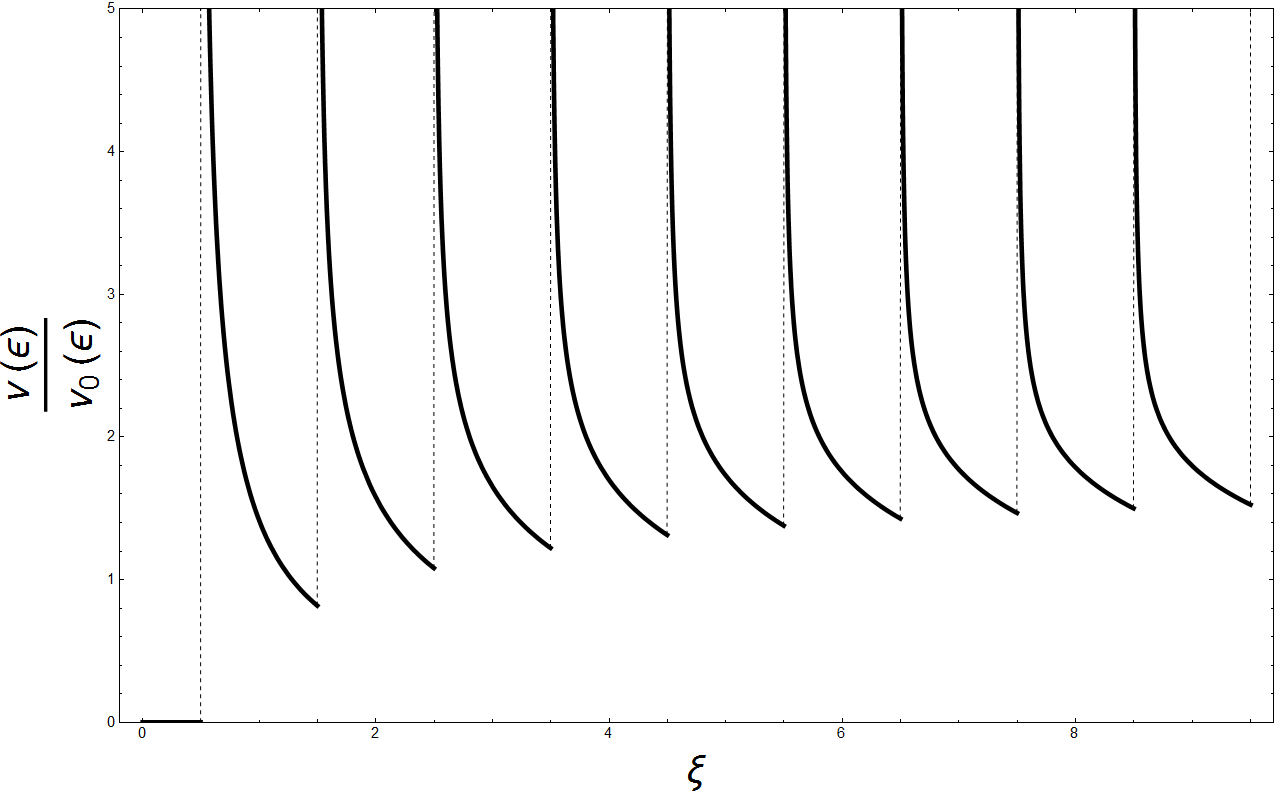
\includegraphics[width=1.0\textwidth]{Figure.png}
\caption{A plot of the ratio of density of states for diamagnetism, $\nu(\varepsilon)$, to a free electron density of states, $\nu_0(\varepsilon)$, versus the quantity $\xi=\varepsilon/\hbar\omega_c$.}
\label{Figure}
\end{figure}

\item Using the result from part (a) we are able to calculate the density of the system
by integrating where we approximate the temperature to be small so that 
\begin{align*}
n = \frac{N}{V} &= \frac{1}{V}\int_{0}^{\infty}\nu(\varepsilon)f(\varepsilon)d\varepsilon\\
&= \frac{1}{4\pi^2}\left(\frac{2m}{\hbar^2}\right)^{3/2}\hbar\omega_c\sum_{l=0}^{\mu/\hbar\omega_c}\int_{0}^{\infty}\left(\varepsilon-\hbar\omega_c\left(l+\frac{1}{2}\right)\right)^{-1/2}\frac{1}{e^{(\varepsilon-\hbar\omega_c(l+1/2)-\mu)/T}+1}d\varepsilon\\
&= \frac{1}{4\pi^2}\left(\frac{2m}{\hbar^2}\right)^{3/2}\hbar\omega_c\sum_{l=0}^{\mu/\hbar\omega_c}\left[2\left(\mu-\hbar\omega_c\left(l+\frac{1}{2}\right)\right)^{1/2} - \frac{\pi^2T^2}{12}\left(\mu-\hbar\omega_c\left(l+\frac{1}{2}\right)\right)^{-3/2}\right]\\
&= \frac{1}{2\pi^2}\left(\frac{2m}{\hbar^2}\right)^{3/2}\hbar\omega_c\sum_{l=0}^{\mu/\hbar\omega_c}\left(\mu-\hbar\omega_c\left(l+\frac{1}{2}\right)\right)^{1/2}\left[1 - \frac{\pi^2T^2}{24}\left(\mu-\hbar\omega_c\left(l+\frac{1}{2}\right)\right)^{-2}\right]
\end{align*}
We see that there exists a singularity for $\mu=\hbar\omega_c(l+1/2)$

\item To find the energy we calculate the integral taking $T=0$ so that
\begin{align*}
E &= \int_{0}^{\infty}\varepsilon\nu(\varepsilon)f(\varepsilon)d\varepsilon\\
&= \frac{1}{4\pi^2}\left(\frac{2m}{\hbar^2}\right)^{3/2}\hbar\omega_c\sum_{l=0}^{\mu/\hbar\omega_c}\int_{0}^{\mu+\hbar\omega_c(1+1/2)}\varepsilon\left(\varepsilon-\hbar\omega_c\left(l+\frac{1}{2}\right)\right)^{-1/2}d\varepsilon\\
&= \frac{1}{4\pi^2}\left(\frac{2m}{\hbar^2}\right)^{3/2}\hbar\omega_c\int_{0}^{\mu}\frac{2\varepsilon^{3/2}}{\hbar\omega_c}+\frac{\hbar\omega_c}{48\varepsilon^{1/2}}d\varepsilon\\
&= \frac{1}{4\pi^2}\left(\frac{2m}{\hbar^2}\right)^{3/2}\hbar\omega_c\left(\frac{4\mu^{5/2}}{5\hbar\omega_c}+\frac{\hbar\omega_c\mu^{1/2}}{24}\right)
\end{align*}
Where we approximated the sum using the \emph{Euler Summation Formula}
$$\sum_{n=0}^{\infty}f(n+1/2) = \int_{0}^{\infty}f(x)dx + \frac{1}{24}f'(0) + ...$$
How taking $d\omega_c/dH=e/mc$ we calculate the magnetism as
\begin{align*}
M = \partiald{E}{H} = \partiald{E}{\omega_c}\partiald{\omega_c}{H} &= \frac{e}{mc}\partiald{}{\omega_c}\left[\frac{1}{4\pi^2}\left(\frac{2m}{\hbar^2}\right)^{3/2}\hbar\omega_c\left(\frac{4\mu^{5/2}}{5\hbar\omega_c}+\frac{\hbar\omega_c\mu^{1/2}}{24}\right)\right]\\
&= \frac{1}{4\pi^2}\left(\frac{2m}{\hbar^2}\right)^{3/2}\frac{\hbar^2\omega_c\mu^{1/2}}{12}\\
&= \frac{1}{12}\nu_0(\mu)\mu_B\hbar\omega_c\\
&= \frac{1}{12}\nu_0(\mu)\mu_B^2H
\end{align*}
\end{enumerate}

\pagebreak

\section{Problem \#3}
\begin{enumerate}[(1)]
\item Given that the cosmic background microwave radiation (CBMR) has a thermal black 
body spectrum at $T=2.72\unit{K}$ we can find the frequency that the spectrum is at a 
maximum by taking \emph{Planck Distribution}
$$E_{\omega} = \frac{V\hbar}{\pi^2c^3}\frac{\omega^3}{e^{-\hbar\omega/T}-1}$$
and finding $\omega_{max}$ which maximizes the distribution. We take a derivative to find
$\omega_{max}$ as
\begin{align*}
\frac{dE}{d\omega} &= \frac{V\hbar}{\pi^2c^3}\left(\frac{3\omega^2}{e^{\hbar\omega/T}-1} - \frac{\hbar}{T}\frac{\omega^3e^{\hbar\omega/T}}{(e^{\hbar\omega/T}-1)^2}\right)\\
&\Downarrow\\
0 &= \frac{3\omega_{max}^2}{e^{\hbar\omega_{max}/T}-1} - \frac{\hbar}{T}\frac{\omega_{max}^3e^{\hbar\omega_{max}/T}}{(e^{\hbar\omega_{max}/T}-1)^2}\\
&\Downarrow\\
3(e^{\hbar\omega_{max}/T}-1) &= \frac{\hbar\omega_{max}}{T}e^{\hbar\omega_{max}/T}\\
&\Downarrow\\
3(1-e^{-\zeta}) &= \zeta
\end{align*}
Where we take 
$$\zeta=\frac{\hbar\omega_{max}}{kT}$$
note that we added the constant $k$ so that we can calculate $\omega_{max}$ from a 
temperature in kelvin. Numerically we find that $\zeta\approx2.822$ so
\begin{align*}
f_{max} = \frac{\omega_{max}}{2\pi} = \zeta\frac{kT}{\hbar} = \frac{2.822}{2\pi}\frac{(1.38\times10^{-23}\unit{J\ K^{-1}})(2.72\unit{K})}{1.05\times10^{-34}\unit{J\ s^{-1}}} = 160\unit{GHz}
\end{align*}

\item If we assume that the radius of the universe changes with time linearly and that the 
expansion for the CBMR is adiabatic which implies that the photon gas undergoes expansion by
$$TV^{1/3} = C$$
where $C$ is a constant. Using this fact we can relate the current temperature of the CBMR
given as $T_c = 2.73\unit{K}$ to the temperature of the universe at one year. Using the fact that
the radius of the universe changes linearly we see that
\begin{align*}
V_0 &= \frac{4}{3}\pi (r_0t_0)^3\\ 
V_c &= \frac{4}{3}\pi r_c^3 = \frac{4}{3}\pi(r_0t_c)^3
\end{align*}
Where $t_c$ is the current age of the universe. So 
\begin{align*}
T_0V_0^{1/3} &=  T_cV_c^{1/3}\\
&\Downarrow\\
T_0 &=  T_ct_c = (2.73\unit{K})\left(\frac{1.4\times10^{10}\unit{yr}}{1\unit{yr}}\right) = 3.8\times10^{10}\unit{K}
\end{align*}
Note we took $t_0=1\unit{yr}$.

\item If we consider the Sun as a black body with a radius of $R = 7.0\times10^{5}\unit{km}$ 
and temperature $T = 6\times10^{3}\unit{K}$ we can calculate the emitted radiation through
the Stefan-Boltzmann constant, $\sigma$, as
\begin{align*}
J_{sun} = \int\sigma T^4d\Omega &= \sigma T^44\pi R^2\\
&= (5.67\times10^{-8}\unit{J\ m^{-2}\ K^{-4}\ s^{-1}})(6\times10^{3}\unit{K})(4\pi)(7.0\times10^{8}\unit{m})\\
&= 4.5\times10^{26}\unit{J\ s^{-1}}
\end{align*}

\item Assuming that the earth is also a black body with the distance between the earth and
sun is $R_o=5\times10^{8}\unit{km}$ and radius of $R_e=6\times10^{3}\unit{km}$ we can
calculate the amount of energy that is absorbed by the earth by noting we assumed the sun
was also a black body in part (3) so the amount of energy propagates without changing in 
phase space. This implies that the earth sees it's cross section a distance $R_o$
\begin{align*}
A_{earth} = J_{sun}\frac{\pi R_E^2}{4\pi R_o^2} &= 4.5\times10^{26}\unit{J\ s^{-1}}\frac{\pi (6\times10^{6}\unit{m})}{4\pi(5\times10^{11}\unit{m})^2}\\
&= 1.35\times10^{21}\unit{J\ s^{1-}}
\end{align*}
Now, due to the assumption that earth is a black body we can take all this energy absorbed
is emitted. Where we integrated over the solid angle 
\begin{align*}
A_{earth} = J_{earth} &= \sigma T^{4}4\pi R_e^2\\
&\Downarrow\\
T &= \frac{A_{earth}}{4\pi\sigma R_e^2} = \frac{1.35\times10^{21}\unit{J\ s^{-1}}}{4\pi(5.67\times10^{-8}\unit{J\ m^{-2}\ K^{-4}\ s^{-1}})(6\times10^{6}\unit{m})^2}\\
&= 287\unit{K}
\end{align*}



\end{enumerate}

\pagebreak

\end{document}

